% Author: Till Tantau
% Source: The PGF/TikZ manual
\documentclass{article}

\usepackage[latin1]{inputenc}
\usepackage{tikz}

% GNUPLOT required
\usepackage{verbatim}

\begin{comment}
:Title: GNUPLOT basics
:Tags: Plots, GNUPLOT, External file

PGF/TikZ provides a convenient mechanism for plotting functions using `GNUPLOT`_.
To run this example for the first time you have to do the following:

- GNUPLOT must be installed on your system. Try typing ``gnuplot`` on the command line to
  see if it's installed. Windows users may have to rename ``wgnuplot`` to ``gnuplot``.
- You must allow TeX to run external programs. The command line option to enable this is
  usually ``--shell-escape`` or ``--enable-write18``
  
PGF will call GNUPLOT for you and store the data in a file. Next time you compile the example,
data will be loaded from the generated file. See section 11.12.3 in the manual for 
more information. 

.. _GNUPLOT: http://www.gnuplot.info/

| Author: Till Tantau
| Source: The PGF/TikZ manual

\end{comment}


\begin{document}
\pagestyle{empty}


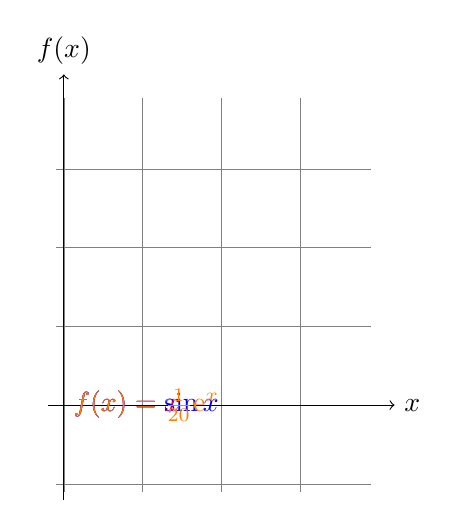
\begin{tikzpicture}[domain=0:4]
    \draw[very thin,color=gray] (-0.1,-1.1) grid (3.9,3.9);
    \draw[->] (-0.2,0) -- (4.2,0) node[right] {$x$};
    \draw[->] (0,-1.2) -- (0,4.2) node[above] {$f(x)$};
    \draw[color=red] plot[id=x] function{x} 
        node[right] {$f(x) =x$};
    \draw[color=blue] plot[id=sin] function{sin(x)} 
        node[right] {$f(x) = \sin x$};
    \draw[color=orange] plot[id=exp] function{0.05*exp(x)} 
        node[right] {$f(x) = \frac{1}{20} \mathrm e^x$};
\end{tikzpicture}


\end{document}